% Author: Izaak Neutelings (September 2021)
% Adapted from 

\documentclass[border=3pt,tikz]{standalone}
\usepackage{amsmath} % for aligned
%\usepackage{amssymb} % for \mathbb
\usepackage{tikz}
%\usepackage{etoolbox} % for \ifthen
\usepackage{listofitems} % for \readlist to create arrays
\usetikzlibrary{arrows.meta} % for arrow size
\usepackage[outline]{contour} % glow around text
\contourlength{1.4pt}

\tikzset{>=latex} % for LaTeX arrow head
%\usepackage{xcolor}

\tikzstyle{node}=[thick,circle,draw=blue,minimum size=22,inner sep=0.5,outer sep=0.6]
\tikzstyle{node in}=[node,green!20!black,draw=green!30!black,fill=green!25]
\tikzstyle{node hidden}=[node,blue!20!black,draw=blue!30!black,fill=blue!20]
\tikzstyle{node out}=[node,red!20!black,draw=red!30!black,fill=red!20]
\tikzstyle{connect}=[thick,black] %,line cap=round
\tikzstyle{connect arrow}=[-{Latex[length=4,width=3.5]},thick,black,shorten <=0.5,shorten >=1]
\tikzset{ % node styles, numbered for easy mapping with \nstyle
  node 1/.style={node in},
  node 2/.style={node hidden},
  node 3/.style={node out},
}
\def\nstyle{int(\lay<\Nnodlen?min(2,\lay):3)} % map layer number onto 1, 2, or 3

\begin{document}

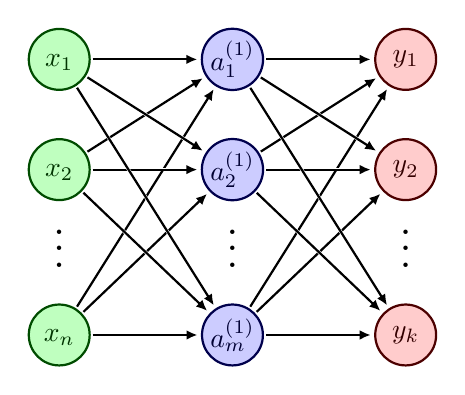
\begin{tikzpicture}[x=2.2cm,y=1.4cm]
  \readlist\Nnod{3,3,3} % array of number of nodes per layer
  \readlist\Nstr{n,m,k} % array of string number of nodes per layer
  \readlist\Cstr{\strut x,a^{(\prev)},y} % array of coefficient symbol per layer
  \def\yshift{0.5} % shift last node for dots
  
  \message{^^J  Layer}
  \foreachitem \N \in \Nnod{ % loop over layers
    \def\lay{\Ncnt} % alias of index of current layer
    \pgfmathsetmacro\prev{int(\Ncnt-1)} % number of previous layer
    \message{\lay,}
    \foreach \i [evaluate={\c=int(\i==\N); \y=\N/2-\i-\c*\yshift;
                 \index=(\i<\N?int(\i):"\Nstr[\lay]");
                 \x=\lay; \n=\nstyle;}] in {1,...,\N}{ % loop over nodes
      % NODES
      \node[node \n] (N\lay-\i) at (\x,\y) {$\Cstr[\lay]_{\index}$};
      
      % CONNECTIONS
      \ifnum\lay>1 % connect to previous layer
        \foreach \j in {1,...,\Nnod[\prev]}{ % loop over nodes in previous layer
          \draw[connect arrow,white,line width=1.2] (N\prev-\j) -- (N\lay-\i);
          \draw[connect arrow] (N\prev-\j) -- (N\lay-\i);
        }
      \fi
      
    }
    \path (N\lay-\N) --++ (0,1+\yshift) node[midway,scale=1.5] {$\vdots$};
  }

\end{tikzpicture}

\end{document}